% Created by tikzDevice version 0.12
% !TEX encoding = UTF-8 Unicode
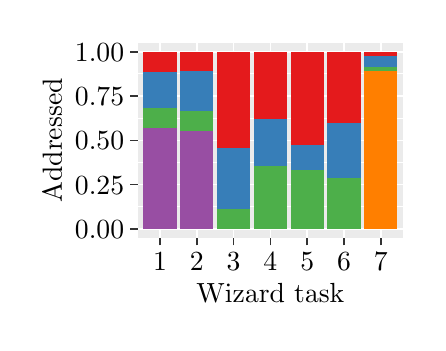
\begin{tikzpicture}[x=1pt,y=1pt]
\definecolor{fillColor}{RGB}{255,255,255}
\path[use as bounding box,fill=fillColor,fill opacity=0.00] (0,0) rectangle (141.12,106.79);
\begin{scope}
\path[clip] (  0.00,  0.00) rectangle (141.12,106.79);
\definecolor{drawColor}{RGB}{255,255,255}
\definecolor{fillColor}{RGB}{255,255,255}

\path[draw=drawColor,line width= 0.6pt,line join=round,line cap=round,fill=fillColor] ( -0.00,  0.00) rectangle (141.12,106.79);
\end{scope}
\begin{scope}
\path[clip] ( 39.80, 30.86) rectangle (135.62,101.29);
\definecolor{fillColor}{gray}{0.92}

\path[fill=fillColor] ( 39.80, 30.86) rectangle (135.62,101.29);
\definecolor{drawColor}{RGB}{255,255,255}

\path[draw=drawColor,line width= 0.3pt,line join=round] ( 39.80, 42.07) --
	(135.62, 42.07);

\path[draw=drawColor,line width= 0.3pt,line join=round] ( 39.80, 58.07) --
	(135.62, 58.07);

\path[draw=drawColor,line width= 0.3pt,line join=round] ( 39.80, 74.08) --
	(135.62, 74.08);

\path[draw=drawColor,line width= 0.3pt,line join=round] ( 39.80, 90.09) --
	(135.62, 90.09);

\path[draw=drawColor,line width= 0.6pt,line join=round] ( 39.80, 34.06) --
	(135.62, 34.06);

\path[draw=drawColor,line width= 0.6pt,line join=round] ( 39.80, 50.07) --
	(135.62, 50.07);

\path[draw=drawColor,line width= 0.6pt,line join=round] ( 39.80, 66.08) --
	(135.62, 66.08);

\path[draw=drawColor,line width= 0.6pt,line join=round] ( 39.80, 82.08) --
	(135.62, 82.08);

\path[draw=drawColor,line width= 0.6pt,line join=round] ( 39.80, 98.09) --
	(135.62, 98.09);

\path[draw=drawColor,line width= 0.6pt,line join=round] ( 47.79, 30.86) --
	( 47.79,101.29);

\path[draw=drawColor,line width= 0.6pt,line join=round] ( 61.10, 30.86) --
	( 61.10,101.29);

\path[draw=drawColor,line width= 0.6pt,line join=round] ( 74.40, 30.86) --
	( 74.40,101.29);

\path[draw=drawColor,line width= 0.6pt,line join=round] ( 87.71, 30.86) --
	( 87.71,101.29);

\path[draw=drawColor,line width= 0.6pt,line join=round] (101.02, 30.86) --
	(101.02,101.29);

\path[draw=drawColor,line width= 0.6pt,line join=round] (114.33, 30.86) --
	(114.33,101.29);

\path[draw=drawColor,line width= 0.6pt,line join=round] (127.64, 30.86) --
	(127.64,101.29);
\definecolor{fillColor}{RGB}{152,78,163}

\path[fill=fillColor] ( 41.80, 34.06) rectangle ( 53.78, 70.44);
\definecolor{fillColor}{RGB}{77,175,74}

\path[fill=fillColor] ( 41.80, 70.44) rectangle ( 53.78, 77.72);
\definecolor{fillColor}{RGB}{55,126,184}

\path[fill=fillColor] ( 41.80, 77.72) rectangle ( 53.78, 90.81);
\definecolor{fillColor}{RGB}{228,26,28}

\path[fill=fillColor] ( 41.80, 90.81) rectangle ( 53.78, 98.09);
\definecolor{fillColor}{RGB}{152,78,163}

\path[fill=fillColor] ( 55.11, 34.06) rectangle ( 67.09, 69.63);
\definecolor{fillColor}{RGB}{77,175,74}

\path[fill=fillColor] ( 55.11, 69.63) rectangle ( 67.09, 76.75);
\definecolor{fillColor}{RGB}{55,126,184}

\path[fill=fillColor] ( 55.11, 76.75) rectangle ( 67.09, 90.98);
\definecolor{fillColor}{RGB}{228,26,28}

\path[fill=fillColor] ( 55.11, 90.98) rectangle ( 67.09, 98.09);
\definecolor{fillColor}{RGB}{77,175,74}

\path[fill=fillColor] ( 68.42, 34.06) rectangle ( 80.39, 41.34);
\definecolor{fillColor}{RGB}{55,126,184}

\path[fill=fillColor] ( 68.42, 41.34) rectangle ( 80.39, 63.17);
\definecolor{fillColor}{RGB}{228,26,28}

\path[fill=fillColor] ( 68.42, 63.17) rectangle ( 80.39, 98.09);
\definecolor{fillColor}{RGB}{77,175,74}

\path[fill=fillColor] ( 81.72, 34.06) rectangle ( 93.70, 56.93);
\definecolor{fillColor}{RGB}{55,126,184}

\path[fill=fillColor] ( 81.72, 56.93) rectangle ( 93.70, 73.70);
\definecolor{fillColor}{RGB}{228,26,28}

\path[fill=fillColor] ( 81.72, 73.70) rectangle ( 93.70, 98.09);
\definecolor{fillColor}{RGB}{77,175,74}

\path[fill=fillColor] ( 95.03, 34.06) rectangle (107.01, 55.41);
\definecolor{fillColor}{RGB}{55,126,184}

\path[fill=fillColor] ( 95.03, 55.41) rectangle (107.01, 64.55);
\definecolor{fillColor}{RGB}{228,26,28}

\path[fill=fillColor] ( 95.03, 64.55) rectangle (107.01, 98.09);
\definecolor{fillColor}{RGB}{77,175,74}

\path[fill=fillColor] (108.34, 34.06) rectangle (120.32, 52.56);
\definecolor{fillColor}{RGB}{55,126,184}

\path[fill=fillColor] (108.34, 52.56) rectangle (120.32, 72.48);
\definecolor{fillColor}{RGB}{228,26,28}

\path[fill=fillColor] (108.34, 72.48) rectangle (120.32, 98.09);
\definecolor{fillColor}{RGB}{255,127,0}

\path[fill=fillColor] (121.65, 34.06) rectangle (133.62, 90.98);
\definecolor{fillColor}{RGB}{77,175,74}

\path[fill=fillColor] (121.65, 90.98) rectangle (133.62, 92.40);
\definecolor{fillColor}{RGB}{55,126,184}

\path[fill=fillColor] (121.65, 92.40) rectangle (133.62, 96.67);
\definecolor{fillColor}{RGB}{228,26,28}

\path[fill=fillColor] (121.65, 96.67) rectangle (133.62, 98.09);
\end{scope}
\begin{scope}
\path[clip] (  0.00,  0.00) rectangle (141.12,106.79);
\definecolor{drawColor}{RGB}{0,0,0}

\node[text=drawColor,anchor=base east,inner sep=0pt, outer sep=0pt, scale=  1.00] at ( 34.85, 30.62) {0.00};

\node[text=drawColor,anchor=base east,inner sep=0pt, outer sep=0pt, scale=  1.00] at ( 34.85, 46.63) {0.25};

\node[text=drawColor,anchor=base east,inner sep=0pt, outer sep=0pt, scale=  1.00] at ( 34.85, 62.63) {0.50};

\node[text=drawColor,anchor=base east,inner sep=0pt, outer sep=0pt, scale=  1.00] at ( 34.85, 78.64) {0.75};

\node[text=drawColor,anchor=base east,inner sep=0pt, outer sep=0pt, scale=  1.00] at ( 34.85, 94.65) {1.00};
\end{scope}
\begin{scope}
\path[clip] (  0.00,  0.00) rectangle (141.12,106.79);
\definecolor{drawColor}{gray}{0.20}

\path[draw=drawColor,line width= 0.6pt,line join=round] ( 37.05, 34.06) --
	( 39.80, 34.06);

\path[draw=drawColor,line width= 0.6pt,line join=round] ( 37.05, 50.07) --
	( 39.80, 50.07);

\path[draw=drawColor,line width= 0.6pt,line join=round] ( 37.05, 66.08) --
	( 39.80, 66.08);

\path[draw=drawColor,line width= 0.6pt,line join=round] ( 37.05, 82.08) --
	( 39.80, 82.08);

\path[draw=drawColor,line width= 0.6pt,line join=round] ( 37.05, 98.09) --
	( 39.80, 98.09);
\end{scope}
\begin{scope}
\path[clip] (  0.00,  0.00) rectangle (141.12,106.79);
\definecolor{drawColor}{gray}{0.20}

\path[draw=drawColor,line width= 0.6pt,line join=round] ( 47.79, 28.11) --
	( 47.79, 30.86);

\path[draw=drawColor,line width= 0.6pt,line join=round] ( 61.10, 28.11) --
	( 61.10, 30.86);

\path[draw=drawColor,line width= 0.6pt,line join=round] ( 74.40, 28.11) --
	( 74.40, 30.86);

\path[draw=drawColor,line width= 0.6pt,line join=round] ( 87.71, 28.11) --
	( 87.71, 30.86);

\path[draw=drawColor,line width= 0.6pt,line join=round] (101.02, 28.11) --
	(101.02, 30.86);

\path[draw=drawColor,line width= 0.6pt,line join=round] (114.33, 28.11) --
	(114.33, 30.86);

\path[draw=drawColor,line width= 0.6pt,line join=round] (127.64, 28.11) --
	(127.64, 30.86);
\end{scope}
\begin{scope}
\path[clip] (  0.00,  0.00) rectangle (141.12,106.79);
\definecolor{drawColor}{RGB}{0,0,0}

\node[text=drawColor,anchor=base,inner sep=0pt, outer sep=0pt, scale=  1.00] at ( 47.79, 19.03) {1};

\node[text=drawColor,anchor=base,inner sep=0pt, outer sep=0pt, scale=  1.00] at ( 61.10, 19.03) {2};

\node[text=drawColor,anchor=base,inner sep=0pt, outer sep=0pt, scale=  1.00] at ( 74.40, 19.03) {3};

\node[text=drawColor,anchor=base,inner sep=0pt, outer sep=0pt, scale=  1.00] at ( 87.71, 19.03) {4};

\node[text=drawColor,anchor=base,inner sep=0pt, outer sep=0pt, scale=  1.00] at (101.02, 19.03) {5};

\node[text=drawColor,anchor=base,inner sep=0pt, outer sep=0pt, scale=  1.00] at (114.33, 19.03) {6};

\node[text=drawColor,anchor=base,inner sep=0pt, outer sep=0pt, scale=  1.00] at (127.64, 19.03) {7};
\end{scope}
\begin{scope}
\path[clip] (  0.00,  0.00) rectangle (141.12,106.79);
\definecolor{drawColor}{RGB}{0,0,0}

\node[text=drawColor,anchor=base,inner sep=0pt, outer sep=0pt, scale=  1.00] at ( 87.71,  7.44) {Wizard task};
\end{scope}
\begin{scope}
\path[clip] (  0.00,  0.00) rectangle (141.12,106.79);
\definecolor{drawColor}{RGB}{0,0,0}

\node[text=drawColor,rotate= 90.00,anchor=base,inner sep=0pt, outer sep=0pt, scale=  1.00] at ( 12.39, 66.08) {Addressed};
\end{scope}
\end{tikzpicture}
